\documentclass[tikz,border=5mm]{standalone}
\usetikzlibrary{positioning, fit}
\usepackage{xcolor}

\begin{document}
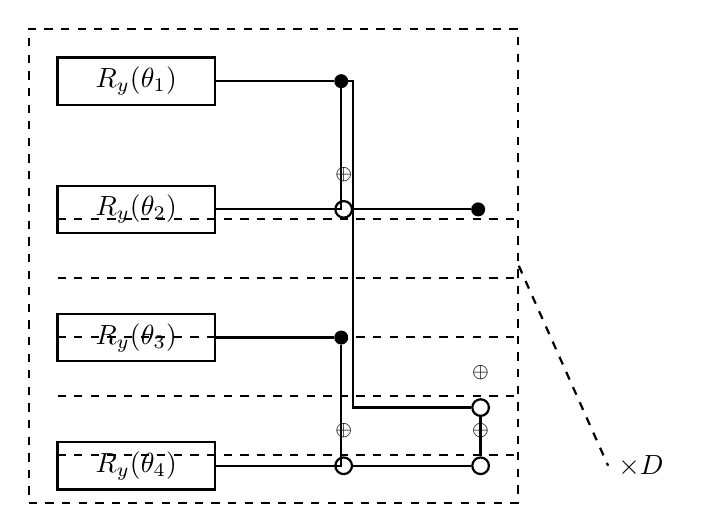
\begin{tikzpicture}[font=\sffamily, thick, >=stealth]

% Define node styles
\tikzset{
  block/.style={draw, rectangle, minimum width=2cm, minimum height=0.6cm, align=center},
  dot/.style={circle, draw, fill, inner sep=1.5pt},
  plus/.style={circle, draw, minimum size=6pt, inner sep=0pt, label={[label distance=0.1cm]\scriptsize $\oplus$}},
  dashedbox/.style={draw, dashed, thick, inner sep=10pt}
}

% Place nodes
\node[block] (R1) at (0,0) {$R_y(\theta_1)$};
\node[block, below=of R1] (R2) {$R_y(\theta_2)$};
\node[block, below=of R2] (R3) {$R_y(\theta_3)$};
\node[block, below=of R3] (R4) {$R_y(\theta_4)$};

\node[dot, right=1.5cm of R1] (dot1) {};
\node[plus, right=1.5cm of R2] (plus1) {};
\node[dot, right=1.5cm of R3] (dot2) {};
\node[plus, right=1.5cm of R4] (plus2) {};

\node[dot, right=1.5cm of plus1] (dot3) {};
\node[plus, right=1.5cm of plus2] (plus3) {};

\node[plus, above=0.5cm of plus3] (top_plus) {};

% Draw edges
\draw (R1.east) -- (dot1);
\draw (dot1) |- (plus1);
\draw (R2.east) -- (plus1);
\draw (plus1) -- (dot3);

\draw (R3.east) -- (dot2);
\draw (dot2) |- (plus2);
\draw (R4.east) -- (plus2);
\draw (plus2) -- (plus3);

\draw (top_plus.west) -- ++(-1.5,0) |- (dot1);
\draw (top_plus.south) -- (plus3.north);

% Draw dashed box
\node[dashedbox, fit=(R1) (plus3), inner xsep=10pt, inner ysep=10pt] (fit) {};

% Add multiplication symbol and label
\node[right=1.5cm of plus3, anchor=west] (times_D) {$\times D$};
\draw[dashed] (fit.east) -- (times_D.west);

% Draw horizontal lines
\foreach \y in {-1.75,-2.5,...,-5.25} {
    \draw[dashed] (-1,\y) -- (fit.east|-{-1,\y});
}

\end{tikzpicture}
\end{document}